%\documentclass[10pt,aspectratio=43,t,l]{beamer}
\documentclass[10pt,aspectratio=169,t,l,fleqn,mathsanserif,sanserif]{beamer}
%\documentclass[10pt]{beamer}

%\setbeamertemplate{footline}[page number]{}

\usepackage{framed}
\usepackage{tcolorbox}
\colorlet{shadecolor}{blue!15}
\usepackage{color,amsmath,xmpmulti,textpos,comment,eurosym,bm,amsthm,tabularx,cancel}
\usepackage{epsfig}
\usepackage{nicefrac}
\usepackage{listings}
%\usepackage{enumitem}
\usepackage{graphicx}    
\usepackage{graphics}
\usepackage{epstopdf}
\usepackage[normalem]{ulem}
\usepackage{float}
%\usepackage[cmbold]{mathtime}
%\usepackage{mt11p}
\usepackage{placeins}
\usepackage{amsmath}
\usepackage{pifont}
\usepackage{color}
\usepackage{amssymb}
\usepackage{mathtools}
\usepackage{subfigure}
\usepackage{multirow}
\usepackage{epsfig}
\usepackage{listings}
%\usepackage{enumitem}
\usepackage{rotating,tabularx}
%\usepackage[graphicx]{realboxes}
\usepackage{graphicx}
\usepackage{graphics}
\usepackage{epstopdf}
\usepackage{longtable}
%\usepackage[pdftex]{hyperref}
\usepackage{breakurl}
\usepackage{epigraph}
\usepackage{xspace}
\usepackage{amsfonts}
\usepackage{eurosym}
\usepackage{ulem}
\usepackage{footmisc}
\usepackage{comment}
\usepackage{setspace}
\usepackage{geometry}
\usepackage{caption}
\usepackage{pdflscape}
\usepackage{array}
\usepackage[round]{natbib}
\usepackage{booktabs}
\usepackage{dcolumn}
\usepackage{mathrsfs}
\usepackage{tikz}
\usetikzlibrary{decorations.pathreplacing}
\usepackage{sansmathaccent}
\pdfmapfile{+sansmathaccent.map}
\usetikzlibrary{shapes.geometric, arrows,chains}
\tikzset{
  startstop/.style={
    rectangle, 
    rounded corners,
    minimum width=3cm, 
    minimum height=1cm,
    align=center, 
    draw=black, 
    fill=red!30
    },
  startsleft/.style={
    rectangle, 
    rounded corners,
    minimum width=3cm, 
    minimum height=1cm,
    align=left, 
    draw=black, 
    fill=red!30
    },
  startsright/.style={
    rectangle, 
    rounded corners,
    minimum width=3cm, 
    minimum height=1cm,
    align=right, 
    draw=black, 
    fill=red!30
    },
  process/.style={
    rectangle, 
    minimum width=3cm, 
    minimum height=1cm, 
    align=center, 
    draw=black, 
    fill=blue!30
    },
  decision/.style={
    rectangle, 
    minimum width=3cm, 
    minimum height=1cm, align=center, 
    draw=black, 
    fill=green!30
    },
  arrow/.style={thick,->,>=stealth},
  dec/.style={
    ellipse, 
    align=center, 
    draw=black, 
    fill=green!30
    },
  font={\fontsize{9pt}{12}\selectfont}
}
%\renewcommand{\labelitemi}{$\blacktriangleright$}

\epstopdfsetup{outdir=./}

\newcolumntype{Y}{>{\centering\arraybackslash}X}
\def\Put(#1,#2)#3{\leavevmode\makebox(0,0){\put(#1,#2){#3}}}

\newcommand{\subhead}[1]{\mbox{}\newline\textbf{#1}\newline}
\newcommand{\ave}[1]{\left\langle #1 \right \rangle}
\newcommand{\eg}{{\it e.g.}}
\newcommand{\ie}{{\it i.e.}}
\newcommand{\cf}{{\it c.f.}}
\newcommand{\etc}{{\it etc.}}
\newcommand{\etal}{{\it et al.}}
%\newcommand{\btVFill}{\vskip0pt plus 1filll}

\newcommand{\del}{D}
\newcommand{\hor}{H}

\newcommand{\threepartdef}[6]
{
  \left\{
    \begin{array}{lll}
      #1 & \mbox{if } #2 \\
      #3 & \mbox{if } #4 \\
      #5 & \mbox{if } #6
    \end{array}
  \right.
}


\newcommand{\Ito}{It\^{o}}
\newcommand{\SP}{S{\&}P500}
\newcommand{\lopt}{\ell_{\text{opt}}}
\newcommand{\gest}{g_{\text{N,T}}}
\newcommand{\elabel}[1]{\label{eq:#1}}
\newcommand{\eref}[1]{Eq.~(\ref{eq:#1})}
\newcommand{\Eref}[1]{Equation~(\ref{eq:#1})}

\newcommand{\flabel}[1]{\label{fig:#1}}
\newcommand{\fref}[1]{Fig.~\ref{fig:#1}}
\newcommand{\Fref}[1]{Figure~\ref{fig:#1}}
\newcommand{\person}[1]{{#1}}
\newcommand{\ra}[1]{\renewcommand{\arraystretch}{#1}}
\newcommand{\vs}[1]{\vspace{.#1cm}}
\newcommand{\vf}{\vspace{.25cm}}
\newcommand{\vff}{\vspace{.6cm}}
\newcommand{\np}{\\ \vf}
\newcommand{\npp}{\\ \vff}
\newcommand{\be}{\begin{equation*}}
\newcommand{\ee}{\end{equation*}}
\newcommand{\bea}{\begin{eqnarray*}}
\newcommand{\eea}{\end{eqnarray*}}
\newcommand{\bc}{\begin{center}}
\newcommand{\ec}{\end{center}}
\newcommand{\bie}{\begin{enumerate}}
\newcommand{\eie}{\end{enumerate}}
\newcommand{\bi}{\begin{itemize}}
\newcommand{\ei}{\end{itemize}}
\newcommand{\toinf}{\rightarrow\infty}
\newcommand{\D}{{\Delta}}
\newcommand{\Dx}{{\Delta x}}
\newcommand{\Dy}{{\Delta y}}
\newcommand{\Du}{{\Delta u}}
\newcommand{\DW}{{\Delta W}}
\newcommand{\DU}{{\Delta U}}
\newcommand{\du}{{\delta u}}
\newcommand{\Dv}{{\Delta v}}
\newcommand{\dt}{{\delta t}}
\newcommand{\gens}{g_{\ave{\,}}}
\newcommand{\ft}[1]{\frametitle{#1}}
\newcommand{\bq}{\begin{quote}}
\newcommand{\eq}{\end{quote}}
\newcommand{\ww}[1]{\bq{\small\rm#1\\}\eq}
\newcommand{\E}{\mathrm{E}}
\newcommand{\Var}{\mathrm{Var}}
\newcommand{\Cov}{\mathrm{Cov}}
\newcommand{\sgn}{\mathrm{sgn}}
\newcommand{\prob}[1]{\mathcal{P}\left(#1\right)}
\newcommand{\lra}{\longrightarrow}
\newcommand{\eps}{\varepsilon}
\newcommand{\ga}{g_\text{ave}}
\newcommand{\gt}{g_\text{typ}}
\newcommand{\gbar}{\bar{g}}
\newcommand{\mbar}{\bar{m}}
\newcommand{\red}[1]{\textcolor{red}{#1}}
\newcommand{\xf}{{x_F}}
\newcommand{\xb}{{x_B}}
\newcommand{\muf}{{\mu_F}}
\newcommand{\mub}{{\mu_B}}
\newcommand{\sigf}{{\sigma_F}}
\newcommand{\sigb}{{\sigma_B}}
\newcommand{\gf}{{\gbar_F}}
\newcommand{\gb}{{\gbar_B}}
\newcommand{\pa}{\textit{pa}}
\newcommand{\taus}{{\tau_\text{s}}}
\newcommand{\Dt}{\Delta t}
\newcommand{\etau}{\tau^\text{eqm}}
\newcommand{\taue}{\tau^\text{EGBM}}
\newcommand{\wtau}{\widetilde{\tau}}
\newcommand{\xN}{\ave{x}_N}
\newcommand{\Sdata}{S^{\text{data}}}
\newcommand{\Smodel}{S^{\text{model}}}
\beamertemplatenavigationsymbolsempty

\newcommand{\tlabel}[1]{\label{tab:#1}}
\newcommand{\tref}[1]{Tab.~\ref{tab:#1}}
\newcommand{\Tref}[1]{Table~\ref{tab:#1}}

\newenvironment{myindentpar}[1]%
{\begin{list}{}%
    {\setlength{\leftmargin}{#1}}%
  \item[]%
}
{\end{list}}

%\usetheme[width=1.8cm,hideothersubsections]{Frankfurt}
\usetheme{Frankfurt}

\newcommand\BackgroundPicture[1]{
\setbeamertemplate{background}{
\parbox[c][\paperheight]{\paperwidth}{
\vfill \hfill
\includegraphics[width=1\paperwidth,height=1\paperheight]{#1}
\hfill \vfill
}}}


\definecolor{lmlblue}{RGB}{0,77,123}
\definecolor{deepblue}{RGB}{35,33,169}
\definecolor{lmllb}{RGB}{237,244,255}
\definecolor{lmlred}{RGB}{155,29,29}
\definecolor{lmlgrey}{RGB}{142,142,142}
\definecolor{lmlgrey2}{RGB}{82,82,82}
\definecolor{grey}{RGB}{210,210,210}
\xdefinecolor{lightblue}{rgb}{0,200,255}
\setbeamercolor{important}{bg=lightblue,fg=red}
\AtBeginEnvironment{definition}{%
  \setbeamercolor{block body}{fg=black,bg=white}
  \setbeamercolor{block title}{bg=lmllb,fg=black}
}

\AtBeginEnvironment{theorem}{%
  \setbeamercolor{block body}{fg=black,bg=white}
  \setbeamercolor{block title}{bg=lmllb,fg=black}
}

%\newcommand{\propnumber}{} % initialize
%\newtheorem*{prop}{Proposition \propnumber}
%\newenvironment{propc}[1]
%  {\renewcommand{\propnumber}{#1}%
%   \begin{shaded}\begin{prop}}
%  {\end{prop}\end{shaded}}
%\AtBeginEnvironment{propc}{%
%  \setbeamercolor{block body}{fg=black,bg=white}
%  \setbeamercolor{block title}{bg=lmllb,fg=black}
%}

\setbeamercolor{fine separation line}{fg=lmllb}

\setbeamercolor{item projected}{fg=white, bg=black}

\setbeamercolor{frametitle}{bg=lmllb, fg=black}
\setbeamertemplate{frametitle}[default][left,colsep=-4bp,rounded=false,shadow=false]

\setbeamercolor{structure}{bg=white, fg=black}
%structure changes color of title in sidebar.

%\setbeamertemplate{frametitle}[default][colsep=-4bp,rounded=false,shadow=false]
\setbeamercolor{section in head/foot}{fg=lmlgrey2, bg=lmllb}
\setbeamercolor{normal text}{fg=black}
\setbeamercolor{title}{bg=white,fg=deepblue}

\hypersetup{colorlinks,linkcolor=,urlcolor=deepblue}

\setbeamerfont{title in sidebar}{size=\fontsize{9}{9}\selectfont}
\setbeamerfont{section in sidebar}{size=\fontsize{7}{7}\selectfont}

% add frame numbers to navigation bar
% (for RSS 2015 conference)
\addtobeamertemplate{navigation symbols}{}{
    \usebeamerfont{footline}
    \usebeamercolor[fg]{footline}
    \hspace{1em}
    \scriptsize
%    \insertframenumber/\inserttotalframenumber
}
\setbeamertemplate{navigation symbols}{} %gets rid of navigation symbols
\setbeamercovered{transparent=20}
%\setbeamertemplate{footline}[frame number] % to show overlay page numbers type: page number
%\setbeamersize{text margin left=0.65cm, text margin right=0.65cm}
%\setbeamercolor{item}{fg=black!70!black} % red bullets
%\setbeamertemplate{itemize subitem}[triangle] % triangle sub-bullets
%\setbeamerfont{itemize/enumerate subbody}{size=\normalsize}


\title[\begin{flushleft} \color{white} {\tiny ???} \end{flushleft}]{\bf {Industrial Organization, Week 3 \\ 
Oligopoly}}
\author[shortname]{ Dio Mavroyiannis \inst{\dag}}
\institute[\begin{flushleft} \color{white} {\large ???} \end{flushleft}]{Milestone Institute}
%\institute[shortinst]{\inst{*} London Mathematical Laboratory \and \inst{\dag} Universit\'{e} Paris-Dauphine \and \inst{\ddag} London Mathematical Laboratory and Santa Fe Institute}
\date{17 February 2021}

\AtBeginSection[]{
\frame{
\ft{Agenda}
\tableofcontents[currentsection,hideallsubsections]
}
}

\makeatletter
\setbeamertemplate{headline}{%
  \pgfuseshading{beamer@barshade}%
  \ifbeamer@sb@subsection%
    \vskip-9.75ex%
  \else%
    \vskip-7ex%
  \fi%
    \begin{beamercolorbox}[ht=3.5ex,dp=2.125ex]{section in head/foot}
     \insertsectionnavigationhorizontal{\textwidth}{}{}%
  \end{beamercolorbox}%
  \ifbeamer@sb@subsection%
    \begin{beamercolorbox}[ignorebg,ht=2.125ex,dp=1.125ex,%
      leftskip=.3cm,rightskip=.3cm plus1fil]{subsection in head/foot}
      \usebeamerfont{subsection in head/foot}\insertsubsectionhead
    \end{beamercolorbox}%
  \fi%
}%

\makeatother

\setbeamertemplate{mini frames}{}
\setbeamertemplate{itemize items}[triangle]

\begin{document}
\frame{\titlepage\insertlogo}

\section{Big picture}
%%%%%%%%%%%%%%%%%%%%%%%%%%%%%%%%%%%%%%%%%%%%%
\frame{\ft{Demand in price competition}
\setbeamertemplate{itemize items}[triangle]

\bi
\item A monopolist sets the monopoly price and quantity, regardless controlling prices or quantities
\item Oligopoly means a few firms, implicitly there is some cost to enter the industry
\item Nash equilibrium in industrial organization implies a reaction function
\item Reaction function: Reacting to the other players reaction. 
\item Example: Quantity competitionm, $q_i(q_{-i})$
\item Ultimately the question is about demand elasticity.
\ei

}

\section{Oligopoly: Quantity}

%%%%%%%%%%%%%%%%%%%%%%%%%%%%%%%%%%%%%%%%%%%%%
\frame{\ft{Antoine-Augustin Cournot}
\setbeamertemplate{itemize items}[triangle]

\bi
\item French Mathematician, Born in 1801, Sorbonne
\item Book:'Recherches sur les principes mathématiques de la théorie des richesses', 1838
\ei

\begin{picture}(80,80)(0,0) %syntax: \begin{picture}(width,height)(x-offset,y-offset)
\put(50,-90){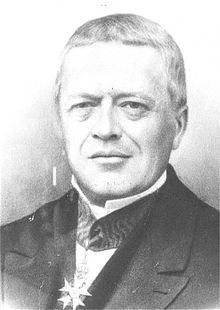
\includegraphics[width=4cm]{./IO_Week3_Quantity_Cournot.jpg}}
\end{picture}

}
%%%%%%%%%%%%%%%%%%%%%%%%%%%%%%%%%%%%%%%%%%%%%

\frame{\ft{Demand in quantity competition}
\setbeamertemplate{itemize items}[triangle]

$
P(Q) = P(q_1,q_2,q_3,...,q_n)  
$

Example: $P(Q) = 100-Q$

\bi
\item Note 1: An asymmetric equilibrium is often(not always) not an option because there exists a deviation
\item Suppose firm 1 is producing 10 and firm 2 is producing 100. Firm 2 has a higher incentive than firm 1 to decrease it's quantity because it will increase revenue on 99 units.
\item n is number of firms. We will be using $i$ and $j$ to talk about two different firms
\ei

}


%%%%%%%%%%%%%%%%%%%%%%%%%%%%%%%%%%%%%%%%%%%%%
\frame{\ft{Demand in quantity competition}
\setbeamertemplate{itemize items}[triangle]

\begin{align}
max_q \pi(Q) &= P(Q)q_i- C(q_i) \\
&=(a-bQ)q_i- C(q_i) \\
&=aq-b(q_i+q_j)q-cq_i \\
&=[a-b(q_i+q_j)-c]q_i \\
& \rightarrow q_i = \frac{a-bq_j-c}{2b} = \frac{a-c}{2b}-\frac{q_j}{2}
\end{align}
}
%%%%%%%%%%%%%%%%%%%%%%%%%%%%%%%%%%%%%%%%%%%%%

\frame{\ft{Quantity Reaction Graph}

\setbeamertemplate{itemize items}[triangle]

\begin{picture}(80,80)(0,0) %syntax: \begin{picture}(width,height)(x-offset,y-offset)
\put(30,-120){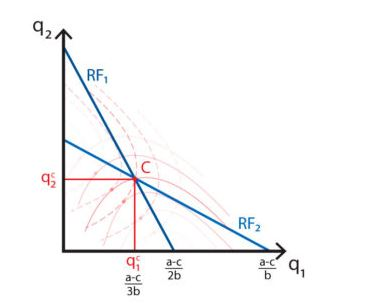
\includegraphics[width=8cm]{./IO_Week3_Quantity_Reaction.jpg}}
\end{picture}

}

\frame{\ft{Herfindahl Index: A measure of market power}

\setbeamertemplate{itemize items}[triangle]

If we have linear costs, we can re-write industry profits as 

\begin{align}
\sum_{i=1}^n \pi = \sum_{i=1}^n (p -c)q_i 
\end{align}

This can be re-written in two equivalent ways.

\begin{align}
(p-\sum_{i=1}^n)q = \frac{p q}{\eta}\sum_{i=1}^n a_i^2 
\end{align}

We simply divide the the total industry profits by the revenue to measure market power

\begin{align}
\frac{1}{\eta}\sum_{i=1}^n a_i^2 
\end{align}


}

\frame{\ft{Lessons from Cournot}
\setbeamertemplate{itemize items}[triangle]


\bi
\item Lesson 1: Profits increase when a firm becomes \textit{relatively} more efficient
\item Lesson 2: Converges to perfect competition as number of firms increases
\item Lesson 3: Markup higher $\leftrightarrow$ higher market share
\item Lesson 4: Less elastic demand means higher markup/profits/market share
\ei

}
%%%%%%%%%%%%%%%%%%%%%%%%%%%%%%%%%%%%%%%%%%%%%
%%%%%%%%%%%%%%%%%%%%%%%%%%%%%%%%%%%%%%%%%%%%%
%%%%%%%%%%%%%%%%%%%%%%%%%%%%%%%%%%%%%%%%%%%%%
%%%%%%%%%%%%%%%%%%%%%%%%%%%%%%%%%%%%%%%%%%%%%
%%%%%%%%%%%%%%%%%%%%%%%%%%%%%%%%%%%%%%%%%%%%%

%%%%%%%%%%%%%%%%%%%%%%%%%%%%%%%%%%%%%%%%%%%%%

\section{Oligopoly: Price}

%%%%%%%%%%%%%%%%%%%%%%%%%%%%%%%%%%%%%%%%%%%%%
\frame{\ft{Joseph Bertrand}
\setbeamertemplate{itemize items}[triangle]

\bi
\item French Mathematician, Born in 1822, Ecole Polytechnique
\item Bertrand, J. (1883) "Book review of théorie mathématique de la richesse sociale and of recherches sur les principles mathematiques de la theorie des richesses", Journal de Savants
\ei

\begin{picture}(80,80)(0,0) %syntax: \begin{picture}(width,height)(x-offset,y-offset)
\put(50,-90){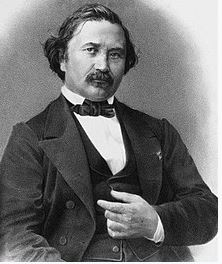
\includegraphics[width=4cm]{./IO_Week3_Quantity_Bertrand.jpg}}
\end{picture}

}
%%%%%%%%%%%%%%%%%%%%%%%%%%%%%%%%%%%%%%%%%%%%%

\frame{\ft{Demand in price competition}
\setbeamertemplate{itemize items}[triangle]

$
Q(p) =
\left\{
  \begin{array}{ll}
     Q(p_i) & \mbox{if } p_i < p_j  \\
    a_i Q(p_i) & \mbox{if }  p_i = p_j \\
    0 & \mbox{if } p_i > p_j 0 \\
  \end{array}
\right.
$

\bi
\item Note 1: If you have a lower price, you get all of the demand
\item Note 2: $a_i$ has to be between 0 and 1 to indicate that the market is split. 
\item Note 3: If consumers prefer the "new" , and firm i enters second then, $a_i>0.5$, if they have $\epsilon$ switching cost $a_i<0.5$
\ei

}
%%%%%%%%%%%%%%%%%%%%%%%%%%%%%%%%%%%%%%%%%%%%%

\frame{\ft{Price Reaction Graph}

\setbeamertemplate{itemize items}[triangle]

\begin{picture}(80,80)(0,0) %syntax: \begin{picture}(width,height)(x-offset,y-offset)
\put(30,-120){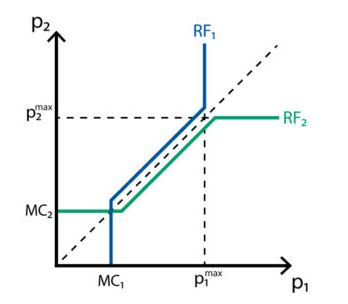
\includegraphics[width=8cm]{./IO_Week3_Price_Reaction.jpg}}
\end{picture}

}
%%%%%%%%%%%%%%%%%%%%%%%%%%%%%%%%%%%%%%%%%%%%%

\frame{\ft{Notes on Bertrand Competition}
\setbeamertemplate{itemize items}[triangle]

\bi
\item Lesson 1: Prices equal to marginal cost
\item Lesson 2: Perfect competition is possible with only two firms
\item Extensions 1: If they do not know each others costs, then weakly expected positive profits
\item Extensions 2: If the products are not homogenous, some market power
\item Extensions 3: If not symmetric, either monopoly price or competitors cost
\ei

}

\section{Comparison}

%%%%%%%%%%%%%%%%%%%%%%%%%%%%%%%%%%%%%%%%%%%%%
\frame{\ft{Comparison}

\setbeamertemplate{itemize items}[triangle]

\bi
\item If product is homogenous. Quantity has higher prices, lower quantities and higher profits
\item If we have a price setting but firms chooses capacity first(at linear cost), results identical
\item High capacity $\rightarrow$ price competition
\item Low capacity $\rightarrow$ quantity competition
\item Alternative framing: what is easier to adjust, prices or quantities?
\item Extension: Even if products are heterogenous, price always gives lower prices and higher quantity
\ei

}

\end{document}